% Use with CC terms.
% Adrin Jalali - 2013
%

\documentclass{beamer}
\setbeamertemplate{navigation symbols}{}

\usepackage{beamerthemeshadow}
\usepackage[absolute,overlay]{textpos}
\usepackage{graphics}

\setbeamercolor{framesource}{fg=gray}
\setbeamerfont{framesource}{size=\tiny}

\newcommand{\source}[1]{\begin{textblock*}{4cm}(8.7cm,8.6cm)
    \begin{beamercolorbox}[ht=0.5cm,right]{framesource}
        \usebeamerfont{framesource}\usebeamercolor[fg]{framesource} credit: {#1}
    \end{beamercolorbox}
\end{textblock*}}


\begin{document}
\title{PPI Networks and Gene Expression}  
\author{Adrin Jalali}
\date{\today} 

\begin{frame}
\titlepage
\end{frame}

%\begin{frame}\frametitle{Table of contents}\tableofcontents
%\end{frame} 

\section{Intro}
\begin{frame}[plain]
  \frametitle{Data}
\begin{figure}
\includegraphics[width=0.7\textwidth]{Affymetrix-microarray}
\end{figure}
\source{en.wikipedia.org}
\note{http://en.wikipedia.org/wiki/DNA_microarray}
\end{frame}

\begin{frame}[plain]
  \frametitle{Van't Veer breast-cancer data}
\begin{figure}
\includegraphics[height=1\textheight]{vantveer-summary}
\end{figure}
\source{Laura J. van 't Veer et.al. Nature, (2002)}
\note{a, Two-dimensional presentation of transcript ratios for 98 breast tumours. There were 4,968 significant genes across the group. Each row represents a tumour and each column a single gene. As shown in the colour bar, red indicates upregulation, green downregulation, black no change, and grey no data available. The yellow line marks the subdivision into two dominant tumour clusters. b, Selected clinical data for the 98 patients in a: BRCA1 germline mutation carrier (or sporadic patient), ER expression, tumour grade 3 (versus grade 1 and 2), lymphocytic infiltrate, angioinvasion, and metastasis status. White indicates positive, black negative and grey denotes tumours derived from BRCA1 germline carriers who were excluded from the metastasis evaluation. The cluster below the yellow line consists of 36 tumours, of which 34 are ER negative (total 39 ER-negative) and 16 are carriers of the BRCA1 mutation (total 18). c, Enlarged portion from a containing a group of genes that co-regulate with the ER- gene (ESR1). Each gene is labelled by its gene name or accession number from GenBank. Contig ESTs ending with RC are reverse-complementary of the named contig EST. d, Enlarged portion from a containing a group of co-regulated genes that are the molecular reflection of extensive lymphocytic infiltrate, and comprise a set of genes expressed in T and B cells. (Gene annotation as in c.)}
\note{http://www.nature.com/nature/journal/v415/n6871/full/415530a.html}
\end{frame}

\begin{frame}[plain]
  \frametitle{Yeast Protein Interaction Network}
\begin{figure}
\includegraphics[width=0.8\textwidth]{yeastProteinInteractionNetwork}
\end{figure}
\note{http://www.bordalierinstitute.com/images/yeastProteinInteractionNetwork.jpg}
\source{http://osf1.gmu.edu/~rcouch/chem665.htm}
\end{frame}


\section{Formulation} 

\begin{frame}
\begin{figure}
\includegraphics[height=1\textheight]{NICK-page1}
\end{figure}
\end{frame}


\begin{frame}
  \frametitle{NICK}
  \begin{columns}
    \begin{column}{0.5\textwidth}
      
      \begin{block}{\tiny{1. SVM modified objective function}}
        \tiny
        \begin{center}
          $\min_{\mathbf{w}, w_0}\left\{\frac{1}{2}\|\mathbf{w}\|^2 + \frac{1}{2}\beta\sum_{(j,k)\in E}(w_j-w_k)^2\right\}$
        \end{center}
        s.t.:
        \begin{center}
          $\forall i \in \{1,\cdots,n\} : (\mathbf{w}\mathbf{x}_i+w_0)y_i\geq 1$
        \end{center}
      \end{block}
      
      \begin{block}{\tiny{3. Dual to Primal}}
        \tiny
        \begin{center}
          $\mathbf{w} = (\mathbf{I} + \beta \mathbf{B})^{-1} \sum_{i = 1}^n \alpha_i y_i \mathbf{x}_i$
        \end{center}
      \end{block}
    \end{column}
    
    \begin{column}{0.5\textwidth}
      \begin{block}{\tiny{2. Dual problem}}
        \tiny
        \begin{center}
          \begin{align*}
            &\max_\alpha\left\{\sum_{i=1}^n\alpha_i-\frac{1}{2}\sum_{i=1}^n\sum_{j=1}^n\alpha_i\alpha_j y_i y_j (\mathbf{x}_i^T\mathbf{L})(\mathbf{L}^T\mathbf{x}_j)\right\}\\
            &\mathbf{L}\mathbf{L}^T=(\mathbf{I}+\beta \mathbf{B})^{-1}\\
            \text{s.t.: }&\\
            &\forall i \in \{1,\cdots,n\}: \sum_{i=1}^n\alpha_iy_i=0\\
            &\forall i \in \{1,\cdots,n\}: \alpha_i \geq 0
          \end{align*}
        \end{center}
      \end{block}
    \end{column}
  \end{columns}
  \source{Ofer Lavi, et.al., Journal of Computational Biology, (2012)}
\end{frame}

\begin{frame}
  \frametitle{NICK Performance Summary}
  \begin{figure}
    \includegraphics[width=0.8\textwidth]{NICK-perfs}
  \end{figure}
  \source{Ofer Lavi, et.al., Journal of Computational Biology, (2012)}
  \note{http://online.liebertpub.com/doi/full/10.1089/cmb.2012.0065}
\end{frame}


\section{Results}
\begin{frame}
\frametitle{Synthesize data}
\begin{enumerate}
\item A random graph
\item Signal nodes: \[ f(n) = \left\{ 
  \begin{array}{l l}
    N(-\mu, 1) & \quad \text{if $n$ is in class $1$}\\
    N(\mu, 1) & \quad \text{if $n$ is in class $2$}
  \end{array} \right.\]
\item Random nodes: \[f(n) = N(0, 1) \]
\item Pathway: 2, 3, or 4 connected signal nodes.
\end{enumerate}
\end{frame}

\begin{frame}[plain]
\frametitle{Synthesized data}
\begin{figure}
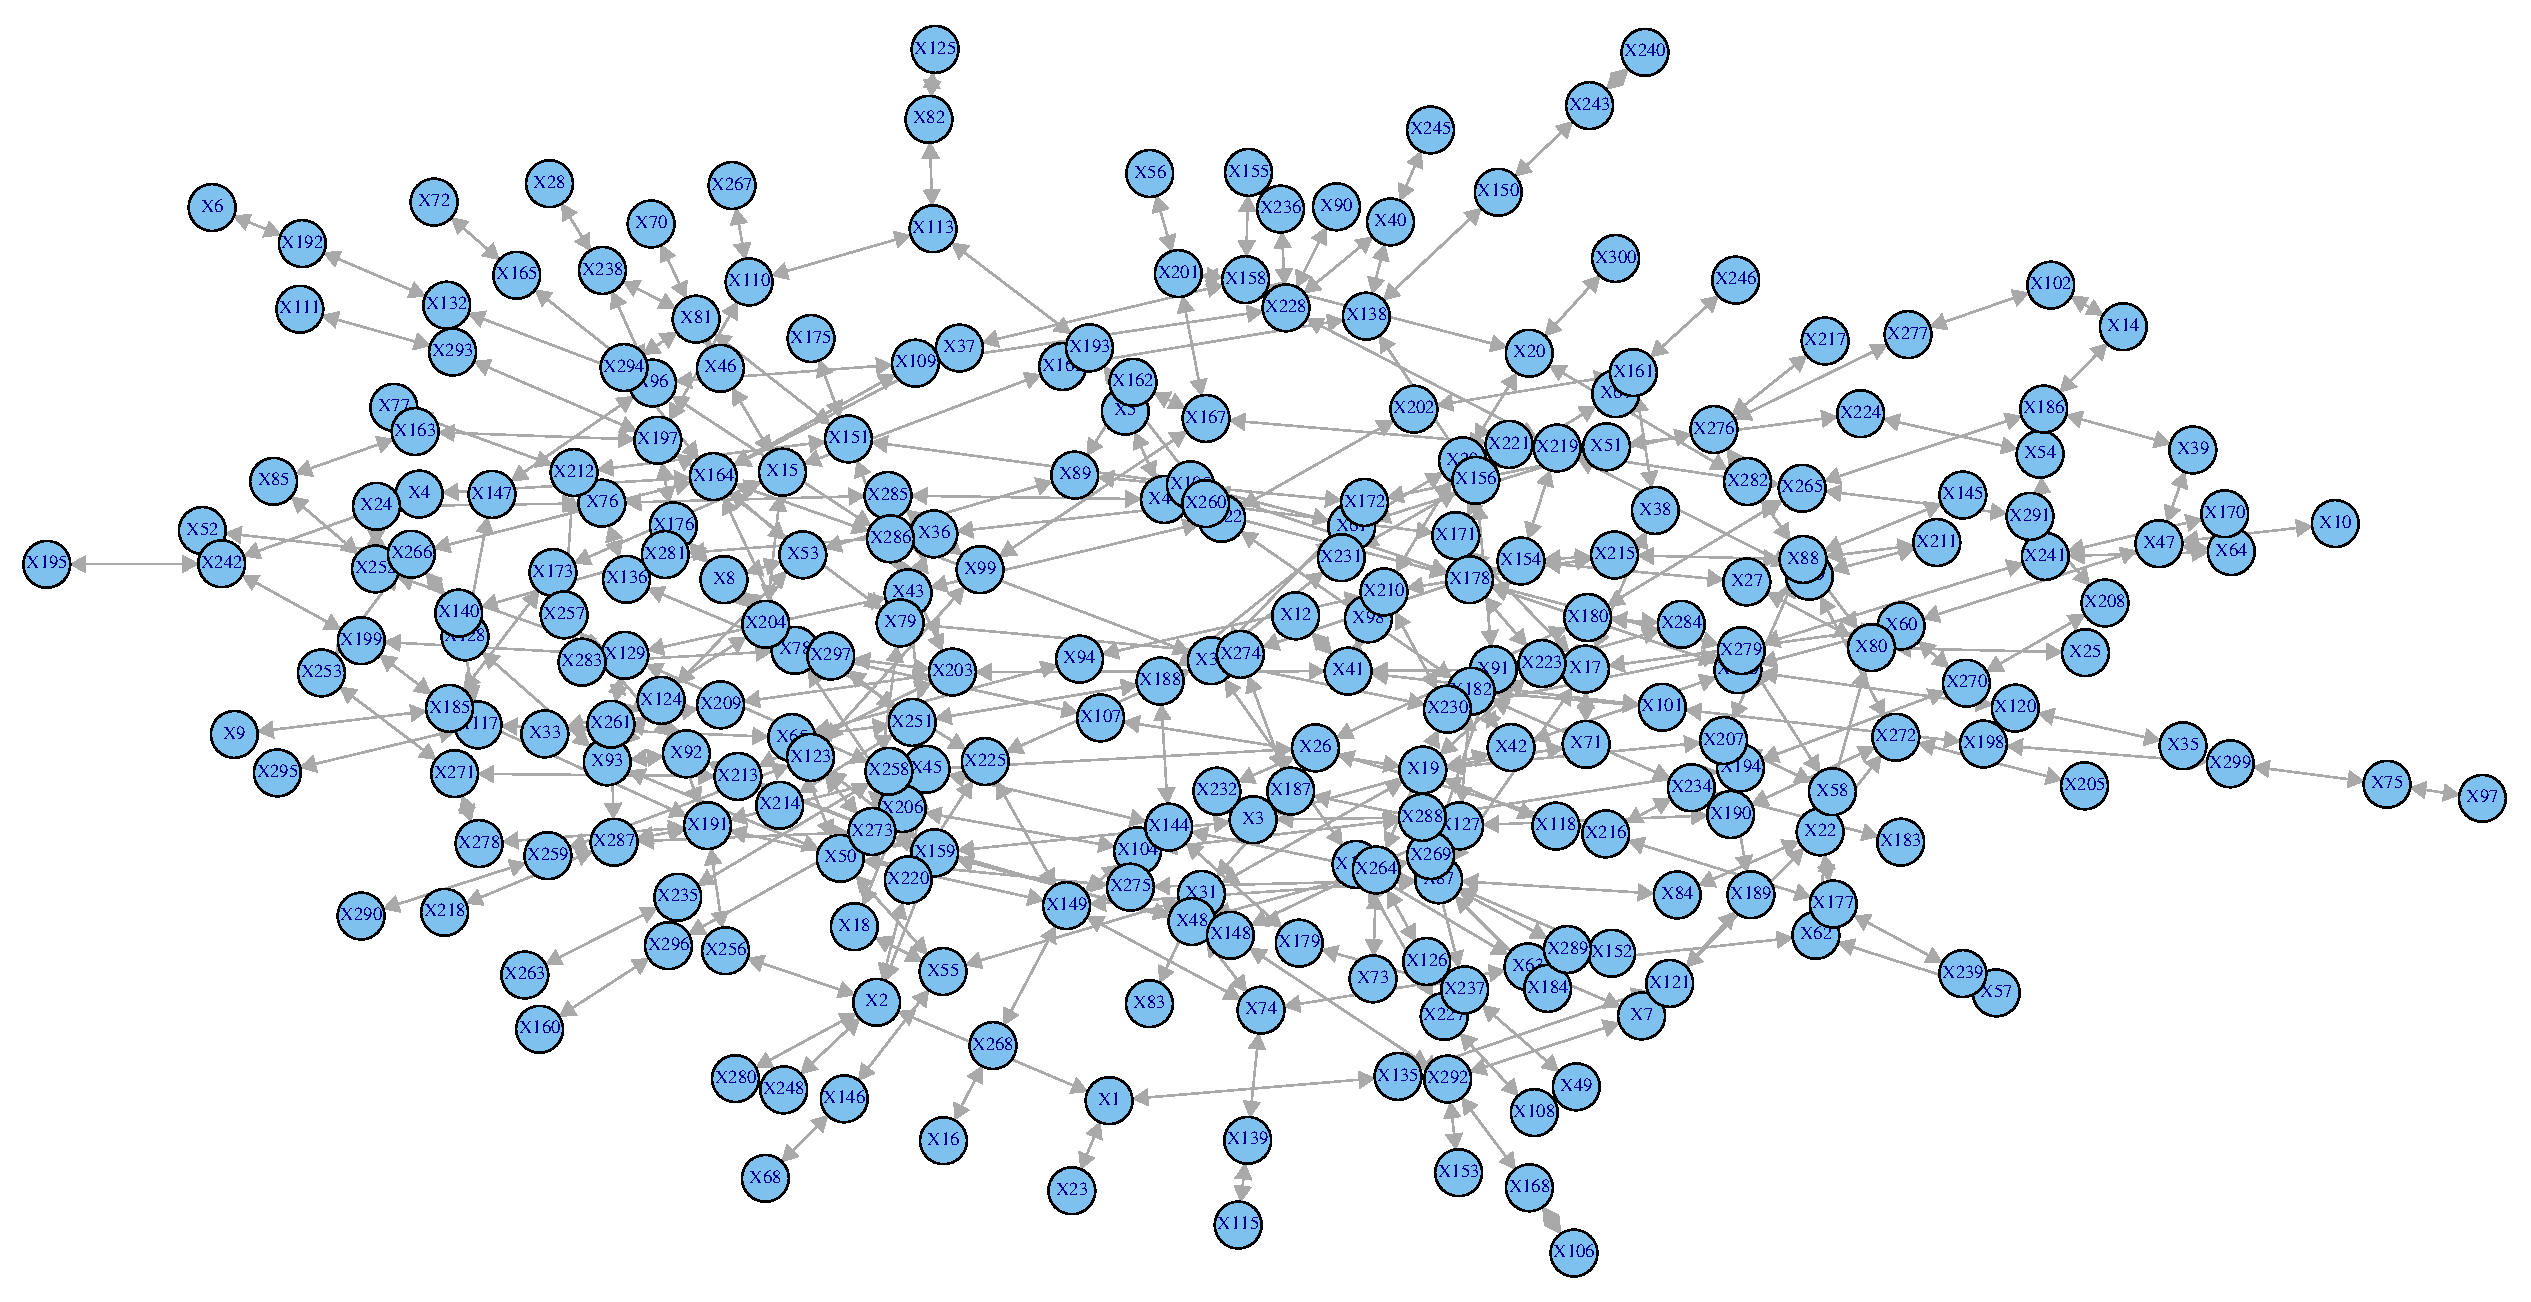
\includegraphics[scale=0.25]{synthesized-graph} 
\end{figure}
\end{frame}

\begin{frame}[plain]
\frametitle{Synthesized data easy scenario}
\begin{figure}
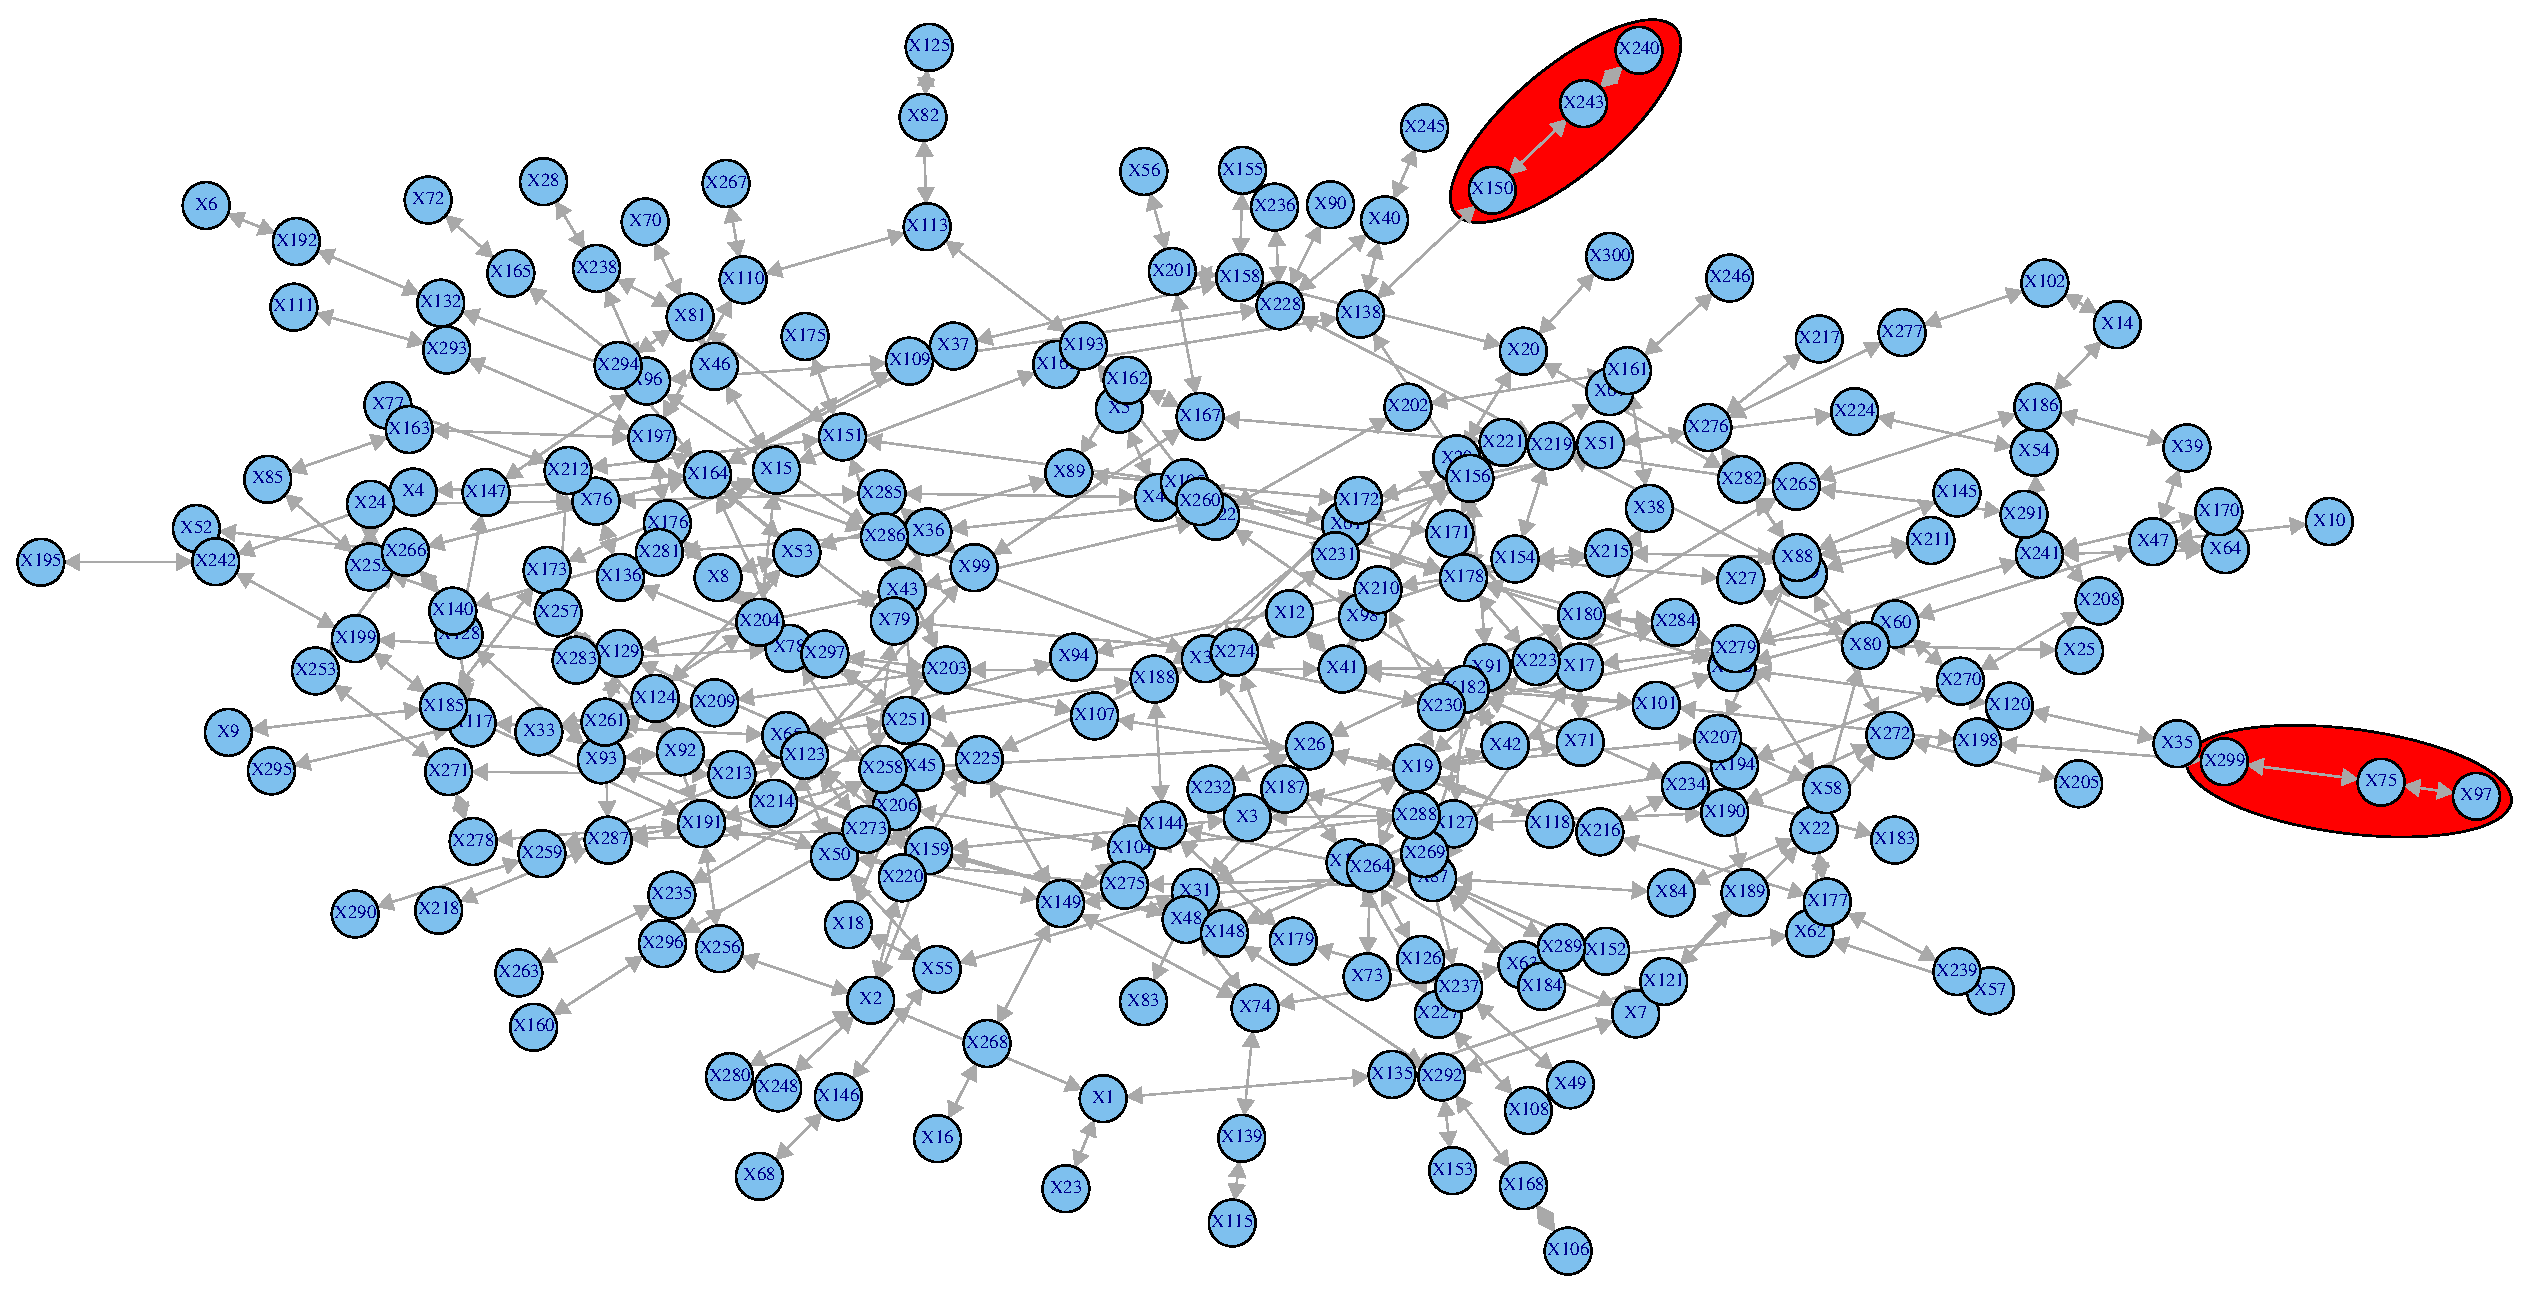
\includegraphics[scale=0.25]{synthesized-graph-easy} 
\end{figure}
\end{frame}

\begin{frame}[plain]
\frametitle{Synthesized data hard scenario}
\begin{figure}
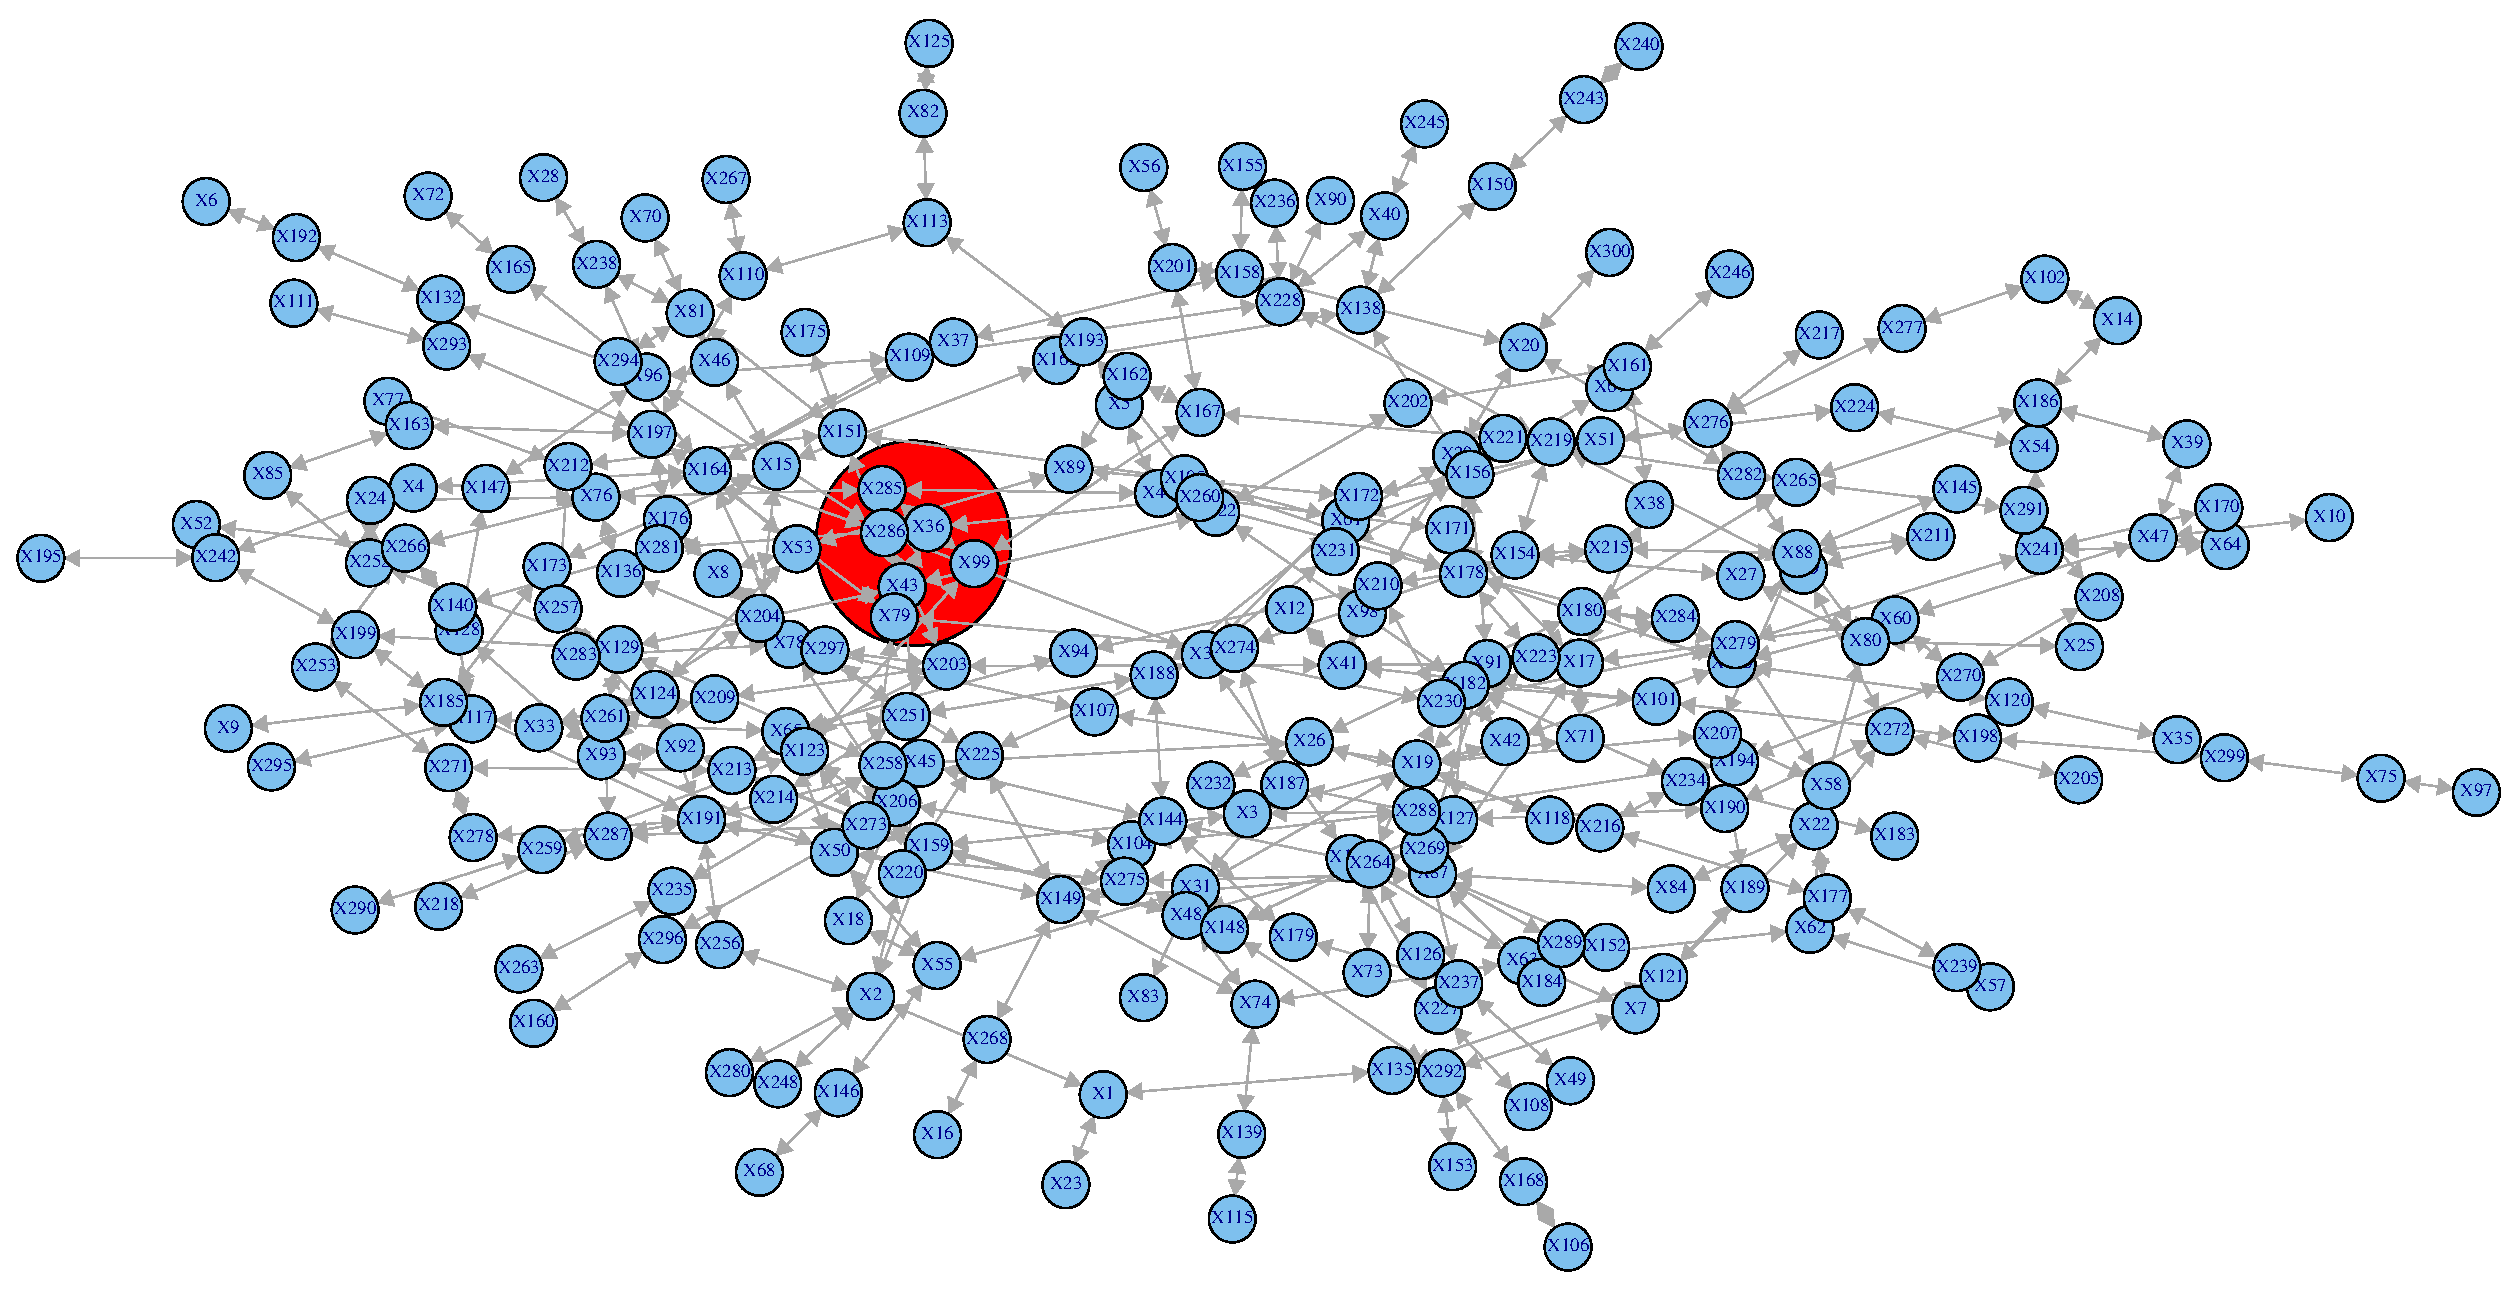
\includegraphics[scale=0.25]{synthesized-graph-hard}
\end{figure}
\end{frame}

\begin{frame}
\frametitle{Results}
\begin{enumerate}
\item Extract pairs of genes with mutual absolute large $w$ 
\item Synthesized easy: all implanted pathways come on top of the list 
\item Synthesized hard: they are vanished \pause
\item Van't veer: 
  \begin{enumerate}
    \item Slightly better performance, although not necessarily as reported.
    \item You find even better genes in w/o network scenario.
    \item Well known genes are of very high degree in the network.
  \end{enumerate}
\end{enumerate}
\end{frame}

\section{Idea}
\begin{frame}
\frametitle{Idea}
\begin{enumerate}
\item Estimate density distribution of each gene for class A. \pause
\item For each sample:
  \begin{enumerate}
  \item Extract abnormal genes according to above estimated distributions.
  \item Extract the part of PPI network induced by extracted genes (almost)
  \end{enumerate}\pause
\item Use a graph kernel for labeled graphs to classify extracted graphs. \pause
\item Extract common sub-graphs from individual graphs that seem to be helping the classification.
\end{enumerate}
\end{frame}

\begin{frame}[plain]
\frametitle{Finished!}
  \begin{center}
    \Huge{Thank You!}
  \end{center}
\end{frame}

\end{document}
